% Options for packages loaded elsewhere
\PassOptionsToPackage{unicode}{hyperref}
\PassOptionsToPackage{hyphens}{url}
%
\documentclass[
]{article}
\title{data exploration}
\author{}
\date{\vspace{-2.5em}}

\usepackage{amsmath,amssymb}
\usepackage{lmodern}
\usepackage{iftex}
\ifPDFTeX
  \usepackage[T1]{fontenc}
  \usepackage[utf8]{inputenc}
  \usepackage{textcomp} % provide euro and other symbols
\else % if luatex or xetex
  \usepackage{unicode-math}
  \defaultfontfeatures{Scale=MatchLowercase}
  \defaultfontfeatures[\rmfamily]{Ligatures=TeX,Scale=1}
  \setmainfont[]{Times New Roman}
\fi
% Use upquote if available, for straight quotes in verbatim environments
\IfFileExists{upquote.sty}{\usepackage{upquote}}{}
\IfFileExists{microtype.sty}{% use microtype if available
  \usepackage[]{microtype}
  \UseMicrotypeSet[protrusion]{basicmath} % disable protrusion for tt fonts
}{}
\makeatletter
\@ifundefined{KOMAClassName}{% if non-KOMA class
  \IfFileExists{parskip.sty}{%
    \usepackage{parskip}
  }{% else
    \setlength{\parindent}{0pt}
    \setlength{\parskip}{6pt plus 2pt minus 1pt}}
}{% if KOMA class
  \KOMAoptions{parskip=half}}
\makeatother
\usepackage{xcolor}
\IfFileExists{xurl.sty}{\usepackage{xurl}}{} % add URL line breaks if available
\IfFileExists{bookmark.sty}{\usepackage{bookmark}}{\usepackage{hyperref}}
\hypersetup{
  pdftitle={data exploration},
  hidelinks,
  pdfcreator={LaTeX via pandoc}}
\urlstyle{same} % disable monospaced font for URLs
\usepackage[margin=1in]{geometry}
\usepackage{color}
\usepackage{fancyvrb}
\newcommand{\VerbBar}{|}
\newcommand{\VERB}{\Verb[commandchars=\\\{\}]}
\DefineVerbatimEnvironment{Highlighting}{Verbatim}{commandchars=\\\{\}}
% Add ',fontsize=\small' for more characters per line
\usepackage{framed}
\definecolor{shadecolor}{RGB}{248,248,248}
\newenvironment{Shaded}{\begin{snugshade}}{\end{snugshade}}
\newcommand{\AlertTok}[1]{\textcolor[rgb]{0.94,0.16,0.16}{#1}}
\newcommand{\AnnotationTok}[1]{\textcolor[rgb]{0.56,0.35,0.01}{\textbf{\textit{#1}}}}
\newcommand{\AttributeTok}[1]{\textcolor[rgb]{0.77,0.63,0.00}{#1}}
\newcommand{\BaseNTok}[1]{\textcolor[rgb]{0.00,0.00,0.81}{#1}}
\newcommand{\BuiltInTok}[1]{#1}
\newcommand{\CharTok}[1]{\textcolor[rgb]{0.31,0.60,0.02}{#1}}
\newcommand{\CommentTok}[1]{\textcolor[rgb]{0.56,0.35,0.01}{\textit{#1}}}
\newcommand{\CommentVarTok}[1]{\textcolor[rgb]{0.56,0.35,0.01}{\textbf{\textit{#1}}}}
\newcommand{\ConstantTok}[1]{\textcolor[rgb]{0.00,0.00,0.00}{#1}}
\newcommand{\ControlFlowTok}[1]{\textcolor[rgb]{0.13,0.29,0.53}{\textbf{#1}}}
\newcommand{\DataTypeTok}[1]{\textcolor[rgb]{0.13,0.29,0.53}{#1}}
\newcommand{\DecValTok}[1]{\textcolor[rgb]{0.00,0.00,0.81}{#1}}
\newcommand{\DocumentationTok}[1]{\textcolor[rgb]{0.56,0.35,0.01}{\textbf{\textit{#1}}}}
\newcommand{\ErrorTok}[1]{\textcolor[rgb]{0.64,0.00,0.00}{\textbf{#1}}}
\newcommand{\ExtensionTok}[1]{#1}
\newcommand{\FloatTok}[1]{\textcolor[rgb]{0.00,0.00,0.81}{#1}}
\newcommand{\FunctionTok}[1]{\textcolor[rgb]{0.00,0.00,0.00}{#1}}
\newcommand{\ImportTok}[1]{#1}
\newcommand{\InformationTok}[1]{\textcolor[rgb]{0.56,0.35,0.01}{\textbf{\textit{#1}}}}
\newcommand{\KeywordTok}[1]{\textcolor[rgb]{0.13,0.29,0.53}{\textbf{#1}}}
\newcommand{\NormalTok}[1]{#1}
\newcommand{\OperatorTok}[1]{\textcolor[rgb]{0.81,0.36,0.00}{\textbf{#1}}}
\newcommand{\OtherTok}[1]{\textcolor[rgb]{0.56,0.35,0.01}{#1}}
\newcommand{\PreprocessorTok}[1]{\textcolor[rgb]{0.56,0.35,0.01}{\textit{#1}}}
\newcommand{\RegionMarkerTok}[1]{#1}
\newcommand{\SpecialCharTok}[1]{\textcolor[rgb]{0.00,0.00,0.00}{#1}}
\newcommand{\SpecialStringTok}[1]{\textcolor[rgb]{0.31,0.60,0.02}{#1}}
\newcommand{\StringTok}[1]{\textcolor[rgb]{0.31,0.60,0.02}{#1}}
\newcommand{\VariableTok}[1]{\textcolor[rgb]{0.00,0.00,0.00}{#1}}
\newcommand{\VerbatimStringTok}[1]{\textcolor[rgb]{0.31,0.60,0.02}{#1}}
\newcommand{\WarningTok}[1]{\textcolor[rgb]{0.56,0.35,0.01}{\textbf{\textit{#1}}}}
\usepackage{graphicx}
\makeatletter
\def\maxwidth{\ifdim\Gin@nat@width>\linewidth\linewidth\else\Gin@nat@width\fi}
\def\maxheight{\ifdim\Gin@nat@height>\textheight\textheight\else\Gin@nat@height\fi}
\makeatother
% Scale images if necessary, so that they will not overflow the page
% margins by default, and it is still possible to overwrite the defaults
% using explicit options in \includegraphics[width, height, ...]{}
\setkeys{Gin}{width=\maxwidth,height=\maxheight,keepaspectratio}
% Set default figure placement to htbp
\makeatletter
\def\fps@figure{htbp}
\makeatother
\setlength{\emergencystretch}{3em} % prevent overfull lines
\providecommand{\tightlist}{%
  \setlength{\itemsep}{0pt}\setlength{\parskip}{0pt}}
\setcounter{secnumdepth}{-\maxdimen} % remove section numbering
\usepackage{booktabs}
\usepackage{longtable}
\usepackage{array}
\usepackage{multirow}
\usepackage{wrapfig}
\usepackage{float}
\usepackage{colortbl}
\usepackage{pdflscape}
\usepackage{tabu}
\usepackage{threeparttable}
\usepackage{threeparttablex}
\usepackage[normalem]{ulem}
\usepackage{makecell}
\usepackage{xcolor}
\ifLuaTeX
  \usepackage{selnolig}  % disable illegal ligatures
\fi

\begin{document}
\maketitle

\begin{Shaded}
\begin{Highlighting}[]
\FunctionTok{library}\NormalTok{(devtools)}
\end{Highlighting}
\end{Shaded}

\begin{verbatim}
## Warning: package 'devtools' was built under R version 4.2.1
\end{verbatim}

\begin{verbatim}
## Loading required package: usethis
\end{verbatim}

\begin{verbatim}
## Warning: package 'usethis' was built under R version 4.2.1
\end{verbatim}

\begin{Shaded}
\begin{Highlighting}[]
\FunctionTok{install\_github}\NormalTok{(}\StringTok{"hughjonesd/huxtable"}\NormalTok{)}
\end{Highlighting}
\end{Shaded}

\begin{verbatim}
## WARNING: Rtools is required to build R packages, but is not currently installed.
## 
## Please download and install Rtools 4.2 from https://cran.r-project.org/bin/windows/Rtools/ or https://www.r-project.org/nosvn/winutf8/ucrt3/.
\end{verbatim}

\begin{verbatim}
## Skipping install of 'huxtable' from a github remote, the SHA1 (3e1fde62) has not changed since last install.
##   Use `force = TRUE` to force installation
\end{verbatim}

\begin{Shaded}
\begin{Highlighting}[]
\CommentTok{\#must run data cleaning code first}
\FunctionTok{library}\NormalTok{(tidyverse)}
\end{Highlighting}
\end{Shaded}

\begin{verbatim}
## -- Attaching packages --------------------------------------- tidyverse 1.3.1 --
\end{verbatim}

\begin{verbatim}
## v ggplot2 3.3.6     v purrr   0.3.4
## v tibble  3.1.7     v dplyr   1.0.9
## v tidyr   1.2.0     v stringr 1.4.0
## v readr   2.1.2     v forcats 0.5.1
\end{verbatim}

\begin{verbatim}
## -- Conflicts ------------------------------------------ tidyverse_conflicts() --
## x dplyr::filter() masks stats::filter()
## x dplyr::lag()    masks stats::lag()
\end{verbatim}

\begin{Shaded}
\begin{Highlighting}[]
\FunctionTok{library}\NormalTok{(knitr)}
\FunctionTok{library}\NormalTok{(kableExtra)}
\end{Highlighting}
\end{Shaded}

\begin{verbatim}
## Warning: package 'kableExtra' was built under R version 4.2.1
\end{verbatim}

\begin{verbatim}
## Warning in !is.null(rmarkdown::metadata$output) && rmarkdown::metadata$output
## %in% : 'length(x) = 3 > 1' in coercion to 'logical(1)'
\end{verbatim}

\begin{verbatim}
## 
## Attaching package: 'kableExtra'
\end{verbatim}

\begin{verbatim}
## The following object is masked from 'package:dplyr':
## 
##     group_rows
\end{verbatim}

\begin{Shaded}
\begin{Highlighting}[]
\FunctionTok{load}\NormalTok{(}\AttributeTok{file=}\StringTok{"headscan\_full"}\NormalTok{)}
\end{Highlighting}
\end{Shaded}

\begin{Shaded}
\begin{Highlighting}[]
\NormalTok{age\_sumstats }\OtherTok{\textless{}{-}}\NormalTok{ headscan\_full }\SpecialCharTok{\%\textgreater{}\%} 
  \FunctionTok{summarise}\NormalTok{(}\AttributeTok{n =} \FunctionTok{n}\NormalTok{(),}
            \AttributeTok{min =} \FunctionTok{min}\NormalTok{(age, }\AttributeTok{na.rm =} \ConstantTok{TRUE}\NormalTok{),}
            \AttributeTok{max =} \FunctionTok{max}\NormalTok{(age, }\AttributeTok{na.rm =} \ConstantTok{TRUE}\NormalTok{),}
            \AttributeTok{mean =} \FunctionTok{mean}\NormalTok{(age, }\AttributeTok{na.rm =} \ConstantTok{TRUE}\NormalTok{),}
            \AttributeTok{sd =} \FunctionTok{sd}\NormalTok{(age, }\AttributeTok{na.rm =} \ConstantTok{TRUE}\NormalTok{),}
            \AttributeTok{se =}\NormalTok{ sd}\SpecialCharTok{/}\FunctionTok{sqrt}\NormalTok{(n),}
            \AttributeTok{quant5th =} \FunctionTok{quantile}\NormalTok{(age, }\FloatTok{0.05}\NormalTok{, }\AttributeTok{na.rm=}\ConstantTok{TRUE}\NormalTok{),}
            \AttributeTok{quant25th =} \FunctionTok{quantile}\NormalTok{(age, }\FloatTok{0.25}\NormalTok{, }\AttributeTok{na.rm=}\ConstantTok{TRUE}\NormalTok{),}
            \AttributeTok{quant50th =} \FunctionTok{quantile}\NormalTok{(age, }\FloatTok{0.50}\NormalTok{, }\AttributeTok{na.rm=}\ConstantTok{TRUE}\NormalTok{),}
            \AttributeTok{quant75th =} \FunctionTok{quantile}\NormalTok{(age, }\FloatTok{0.75}\NormalTok{, }\AttributeTok{na.rm=}\ConstantTok{TRUE}\NormalTok{),}
            \AttributeTok{quant95th =} \FunctionTok{quantile}\NormalTok{(age, }\FloatTok{0.95}\NormalTok{, }\AttributeTok{na.rm=}\ConstantTok{TRUE}\NormalTok{),}
            \AttributeTok{na =} \FunctionTok{sum}\NormalTok{(}\FunctionTok{is.na}\NormalTok{(age)))}

\NormalTok{age\_sumstats }\OtherTok{\textless{}{-}}\NormalTok{ age\_sumstats }\SpecialCharTok{\%\textgreater{}\%} 
  \FunctionTok{mutate}\NormalTok{(}\FunctionTok{across}\NormalTok{(}\FunctionTok{where}\NormalTok{(is.numeric), round, }\DecValTok{2}\NormalTok{))}
            
\NormalTok{age\_sumstats }\SpecialCharTok{\%\textgreater{}\%} 
  \FunctionTok{kbl}\NormalTok{(}\AttributeTok{caption =} \StringTok{"Age SumStats"}\NormalTok{) }\SpecialCharTok{\%\textgreater{}\%} 
  \FunctionTok{kable\_styling}\NormalTok{(}\AttributeTok{bootstrap\_options =} \FunctionTok{c}\NormalTok{(}\StringTok{"striped"}\NormalTok{, }\StringTok{"hover"}\NormalTok{, }\StringTok{"condensed"}\NormalTok{), }\AttributeTok{full\_width =} \ConstantTok{TRUE}\NormalTok{)}
\end{Highlighting}
\end{Shaded}

\begin{table}

\caption{\label{tab:unnamed-chunk-4}Age SumStats}
\centering
\begin{tabu} to \linewidth {>{\raggedleft}X>{\raggedleft}X>{\raggedleft}X>{\raggedleft}X>{\raggedleft}X>{\raggedleft}X>{\raggedleft}X>{\raggedleft}X>{\raggedleft}X>{\raggedleft}X>{\raggedleft}X>{\raggedleft}X}
\hline
n & min & max & mean & sd & se & quant5th & quant25th & quant50th & quant75th & quant95th & na\\
\hline
2017 & 18 & 72 & 36.39 & 11.51 & 0.26 & 19 & 26 & 37 & 46 & 54 & 1\\
\hline
\end{tabu}
\end{table}

\begin{Shaded}
\begin{Highlighting}[]
\NormalTok{raceage\_sumstats }\OtherTok{\textless{}{-}}\NormalTok{ headscan\_full }\SpecialCharTok{\%\textgreater{}\%} 
  \FunctionTok{group\_by}\NormalTok{(race\_eth) }\SpecialCharTok{\%\textgreater{}\%} 
  \FunctionTok{summarise}\NormalTok{(}\AttributeTok{n =} \FunctionTok{n}\NormalTok{(),}
            \AttributeTok{min =} \FunctionTok{min}\NormalTok{(age, }\AttributeTok{na.rm =} \ConstantTok{TRUE}\NormalTok{),}
            \AttributeTok{max =} \FunctionTok{max}\NormalTok{(age, }\AttributeTok{na.rm =} \ConstantTok{TRUE}\NormalTok{),}
            \AttributeTok{mean =} \FunctionTok{mean}\NormalTok{(age, }\AttributeTok{na.rm =} \ConstantTok{TRUE}\NormalTok{),}
            \AttributeTok{sd =} \FunctionTok{sd}\NormalTok{(age, }\AttributeTok{na.rm =} \ConstantTok{TRUE}\NormalTok{),}
            \AttributeTok{se =}\NormalTok{ sd}\SpecialCharTok{/}\FunctionTok{sqrt}\NormalTok{(n),}
            \AttributeTok{quant5th =} \FunctionTok{quantile}\NormalTok{(age, }\FloatTok{0.05}\NormalTok{, }\AttributeTok{na.rm=}\ConstantTok{TRUE}\NormalTok{),}
            \AttributeTok{quant25th =} \FunctionTok{quantile}\NormalTok{(age, }\FloatTok{0.25}\NormalTok{, }\AttributeTok{na.rm=}\ConstantTok{TRUE}\NormalTok{),}
            \AttributeTok{quant50th =} \FunctionTok{quantile}\NormalTok{(age, }\FloatTok{0.50}\NormalTok{, }\AttributeTok{na.rm=}\ConstantTok{TRUE}\NormalTok{),}
            \AttributeTok{quant75th =} \FunctionTok{quantile}\NormalTok{(age, }\FloatTok{0.75}\NormalTok{, }\AttributeTok{na.rm=}\ConstantTok{TRUE}\NormalTok{),}
            \AttributeTok{quant95th =} \FunctionTok{quantile}\NormalTok{(age, }\FloatTok{0.95}\NormalTok{, }\AttributeTok{na.rm=}\ConstantTok{TRUE}\NormalTok{),}
            \AttributeTok{na =} \FunctionTok{sum}\NormalTok{(}\FunctionTok{is.na}\NormalTok{(age)))}

\NormalTok{raceage\_sumstats }\OtherTok{\textless{}{-}}\NormalTok{ raceage\_sumstats }\SpecialCharTok{\%\textgreater{}\%} 
  \FunctionTok{mutate}\NormalTok{(}\FunctionTok{across}\NormalTok{(}\FunctionTok{where}\NormalTok{(is.numeric), round, }\DecValTok{2}\NormalTok{))}
            
\NormalTok{raceage\_sumstats }\SpecialCharTok{\%\textgreater{}\%} 
  \FunctionTok{kbl}\NormalTok{(}\AttributeTok{caption =} \StringTok{"Age SumStats by Race/Ethnicity"}\NormalTok{) }\SpecialCharTok{\%\textgreater{}\%} 
  \FunctionTok{kable\_styling}\NormalTok{(}\AttributeTok{bootstrap\_options =} \FunctionTok{c}\NormalTok{(}\StringTok{"striped"}\NormalTok{, }\StringTok{"hover"}\NormalTok{, }\StringTok{"condensed"}\NormalTok{), }\AttributeTok{full\_width =} \ConstantTok{TRUE}\NormalTok{)}
\end{Highlighting}
\end{Shaded}

\begin{table}

\caption{\label{tab:unnamed-chunk-5}Age SumStats by Race/Ethnicity}
\centering
\begin{tabu} to \linewidth {>{\raggedright}X>{\raggedleft}X>{\raggedleft}X>{\raggedleft}X>{\raggedleft}X>{\raggedleft}X>{\raggedleft}X>{\raggedleft}X>{\raggedleft}X>{\raggedleft}X>{\raggedleft}X>{\raggedleft}X>{\raggedleft}X}
\hline
race\_eth & n & min & max & mean & sd & se & quant5th & quant25th & quant50th & quant75th & quant95th & na\\
\hline
AIAN & 8 & 27 & 56 & 43.25 & 11.78 & 4.17 & 27.70 & 33.50 & 45.5 & 53.00 & 56.00 & 0\\
\hline
Asian & 91 & 18 & 56 & 33.23 & 11.76 & 1.23 & 18.00 & 21.50 & 31.0 & 42.50 & 54.00 & 0\\
\hline
Black & 548 & 18 & 71 & 37.92 & 10.79 & 0.46 & 21.00 & 29.00 & 39.0 & 47.00 & 54.00 & 0\\
\hline
LatinX & 100 & 18 & 55 & 34.63 & 11.93 & 1.19 & 19.00 & 23.00 & 34.0 & 44.50 & 53.10 & 1\\
\hline
NHOPI & 4 & 19 & 40 & 27.00 & 9.76 & 4.88 & 19.15 & 19.75 & 24.5 & 31.75 & 38.35 & 0\\
\hline
Other & 21 & 20 & 72 & 37.48 & 14.75 & 3.22 & 20.00 & 25.00 & 33.0 & 51.00 & 55.00 & 0\\
\hline
PTNS & 5 & 29 & 40 & 36.60 & 4.72 & 2.11 & 30.20 & 35.00 & 39.0 & 40.00 & 40.00 & 0\\
\hline
white & 1240 & 18 & 62 & 36.05 & 11.64 & 0.33 & 19.00 & 25.00 & 36.0 & 46.00 & 54.00 & 0\\
\hline
\end{tabu}
\end{table}

\begin{Shaded}
\begin{Highlighting}[]
\NormalTok{genderage\_sumstats }\OtherTok{\textless{}{-}}\NormalTok{ headscan\_full }\SpecialCharTok{\%\textgreater{}\%} 
  \FunctionTok{group\_by}\NormalTok{(gender) }\SpecialCharTok{\%\textgreater{}\%} 
  \FunctionTok{summarise}\NormalTok{(}\AttributeTok{n =} \FunctionTok{n}\NormalTok{(),}
            \AttributeTok{min =} \FunctionTok{min}\NormalTok{(age, }\AttributeTok{na.rm =} \ConstantTok{TRUE}\NormalTok{),}
            \AttributeTok{max =} \FunctionTok{max}\NormalTok{(age, }\AttributeTok{na.rm =} \ConstantTok{TRUE}\NormalTok{),}
            \AttributeTok{mean =} \FunctionTok{mean}\NormalTok{(age, }\AttributeTok{na.rm =} \ConstantTok{TRUE}\NormalTok{),}
            \AttributeTok{sd =} \FunctionTok{sd}\NormalTok{(age, }\AttributeTok{na.rm =} \ConstantTok{TRUE}\NormalTok{),}
            \AttributeTok{se =}\NormalTok{ sd}\SpecialCharTok{/}\FunctionTok{sqrt}\NormalTok{(n),}
            \AttributeTok{quant5th =} \FunctionTok{quantile}\NormalTok{(age, }\FloatTok{0.05}\NormalTok{, }\AttributeTok{na.rm=}\ConstantTok{TRUE}\NormalTok{),}
            \AttributeTok{quant25th =} \FunctionTok{quantile}\NormalTok{(age, }\FloatTok{0.25}\NormalTok{, }\AttributeTok{na.rm=}\ConstantTok{TRUE}\NormalTok{),}
            \AttributeTok{quant50th =} \FunctionTok{quantile}\NormalTok{(age, }\FloatTok{0.50}\NormalTok{, }\AttributeTok{na.rm=}\ConstantTok{TRUE}\NormalTok{),}
            \AttributeTok{quant75th =} \FunctionTok{quantile}\NormalTok{(age, }\FloatTok{0.75}\NormalTok{, }\AttributeTok{na.rm=}\ConstantTok{TRUE}\NormalTok{),}
            \AttributeTok{quant95th =} \FunctionTok{quantile}\NormalTok{(age, }\FloatTok{0.95}\NormalTok{, }\AttributeTok{na.rm=}\ConstantTok{TRUE}\NormalTok{),}
            \AttributeTok{na =} \FunctionTok{sum}\NormalTok{(}\FunctionTok{is.na}\NormalTok{(age)))}

\NormalTok{genderage\_sumstats }\OtherTok{\textless{}{-}}\NormalTok{ genderage\_sumstats }\SpecialCharTok{\%\textgreater{}\%} 
  \FunctionTok{mutate}\NormalTok{(}\FunctionTok{across}\NormalTok{(}\FunctionTok{where}\NormalTok{(is.numeric), round, }\DecValTok{2}\NormalTok{))}
            
\NormalTok{genderage\_sumstats }\SpecialCharTok{\%\textgreater{}\%} 
  \FunctionTok{kbl}\NormalTok{(}\AttributeTok{caption =} \StringTok{"Age SumStats by Gender"}\NormalTok{) }\SpecialCharTok{\%\textgreater{}\%} 
  \FunctionTok{kable\_styling}\NormalTok{(}\AttributeTok{bootstrap\_options =} \FunctionTok{c}\NormalTok{(}\StringTok{"striped"}\NormalTok{, }\StringTok{"hover"}\NormalTok{, }\StringTok{"condensed"}\NormalTok{), }\AttributeTok{full\_width =} \ConstantTok{TRUE}\NormalTok{)}
\end{Highlighting}
\end{Shaded}

\begin{table}

\caption{\label{tab:unnamed-chunk-6}Age SumStats by Gender}
\centering
\begin{tabu} to \linewidth {>{\raggedright}X>{\raggedleft}X>{\raggedleft}X>{\raggedleft}X>{\raggedleft}X>{\raggedleft}X>{\raggedleft}X>{\raggedleft}X>{\raggedleft}X>{\raggedleft}X>{\raggedleft}X>{\raggedleft}X>{\raggedleft}X}
\hline
gender & n & min & max & mean & sd & se & quant5th & quant25th & quant50th & quant75th & quant95th & na\\
\hline
Female & 1064 & 18 & 71 & 36.75 & 11.57 & 0.35 & 20.00 & 26.0 & 38.0 & 47.00 & 54.0 & 1\\
\hline
Male & 939 & 18 & 72 & 35.97 & 11.48 & 0.37 & 19.00 & 26.0 & 35.0 & 46.00 & 54.1 & 0\\
\hline
Non-binary or Other & 5 & 29 & 43 & 34.00 & 5.48 & 2.45 & 29.40 & 31.0 & 32.0 & 35.00 & 41.4 & 0\\
\hline
Prefer not to say & 1 & 39 & 39 & 39.00 & NA & NA & 39.00 & 39.0 & 39.0 & 39.00 & 39.0 & 0\\
\hline
NA & 8 & 22 & 49 & 39.12 & 9.79 & 3.46 & 24.45 & 33.5 & 41.5 & 46.75 & 49.0 & 0\\
\hline
\end{tabu}
\end{table}

\begin{Shaded}
\begin{Highlighting}[]
\NormalTok{agegroup\_sumstats }\OtherTok{\textless{}{-}}\NormalTok{ headscan\_full }\SpecialCharTok{\%\textgreater{}\%} 
  \FunctionTok{group\_by}\NormalTok{(age\_group) }\SpecialCharTok{\%\textgreater{}\%} 
  \FunctionTok{summarise}\NormalTok{(}\AttributeTok{n =} \FunctionTok{n}\NormalTok{(),}
            \AttributeTok{min =} \FunctionTok{min}\NormalTok{(age, }\AttributeTok{na.rm =} \ConstantTok{TRUE}\NormalTok{),}
            \AttributeTok{max =} \FunctionTok{max}\NormalTok{(age, }\AttributeTok{na.rm =} \ConstantTok{TRUE}\NormalTok{),}
            \AttributeTok{mean =} \FunctionTok{mean}\NormalTok{(age, }\AttributeTok{na.rm =} \ConstantTok{TRUE}\NormalTok{),}
            \AttributeTok{sd =} \FunctionTok{sd}\NormalTok{(age, }\AttributeTok{na.rm =} \ConstantTok{TRUE}\NormalTok{),}
            \AttributeTok{se =}\NormalTok{ sd}\SpecialCharTok{/}\FunctionTok{sqrt}\NormalTok{(n),}
            \AttributeTok{quant5th =} \FunctionTok{quantile}\NormalTok{(age, }\FloatTok{0.05}\NormalTok{, }\AttributeTok{na.rm=}\ConstantTok{TRUE}\NormalTok{),}
            \AttributeTok{quant25th =} \FunctionTok{quantile}\NormalTok{(age, }\FloatTok{0.25}\NormalTok{, }\AttributeTok{na.rm=}\ConstantTok{TRUE}\NormalTok{),}
            \AttributeTok{quant50th =} \FunctionTok{quantile}\NormalTok{(age, }\FloatTok{0.50}\NormalTok{, }\AttributeTok{na.rm=}\ConstantTok{TRUE}\NormalTok{),}
            \AttributeTok{quant75th =} \FunctionTok{quantile}\NormalTok{(age, }\FloatTok{0.75}\NormalTok{, }\AttributeTok{na.rm=}\ConstantTok{TRUE}\NormalTok{),}
            \AttributeTok{quant95th =} \FunctionTok{quantile}\NormalTok{(age, }\FloatTok{0.95}\NormalTok{, }\AttributeTok{na.rm=}\ConstantTok{TRUE}\NormalTok{),}
            \AttributeTok{na =} \FunctionTok{sum}\NormalTok{(}\FunctionTok{is.na}\NormalTok{(age)))}
\end{Highlighting}
\end{Shaded}

\begin{verbatim}
## Warning in min(age, na.rm = TRUE): no non-missing arguments to min; returning
## Inf
\end{verbatim}

\begin{verbatim}
## Warning in max(age, na.rm = TRUE): no non-missing arguments to max; returning
## -Inf
\end{verbatim}

\begin{Shaded}
\begin{Highlighting}[]
\NormalTok{agegroup\_sumstats }\OtherTok{\textless{}{-}}\NormalTok{ agegroup\_sumstats }\SpecialCharTok{\%\textgreater{}\%} 
  \FunctionTok{mutate}\NormalTok{(}\FunctionTok{across}\NormalTok{(}\FunctionTok{where}\NormalTok{(is.numeric), round, }\DecValTok{2}\NormalTok{))}
            
\NormalTok{agegroup\_sumstats }\SpecialCharTok{\%\textgreater{}\%} 
  \FunctionTok{kbl}\NormalTok{(}\AttributeTok{caption =} \StringTok{"Age SumStats by Age Group"}\NormalTok{) }\SpecialCharTok{\%\textgreater{}\%} 
  \FunctionTok{kable\_styling}\NormalTok{(}\AttributeTok{bootstrap\_options =} \FunctionTok{c}\NormalTok{(}\StringTok{"striped"}\NormalTok{, }\StringTok{"hover"}\NormalTok{, }\StringTok{"condensed"}\NormalTok{), }\AttributeTok{full\_width =} \ConstantTok{TRUE}\NormalTok{)}
\end{Highlighting}
\end{Shaded}

\begin{table}

\caption{\label{tab:unnamed-chunk-7}Age SumStats by Age Group}
\centering
\begin{tabu} to \linewidth {>{\raggedright}X>{\raggedleft}X>{\raggedleft}X>{\raggedleft}X>{\raggedleft}X>{\raggedleft}X>{\raggedleft}X>{\raggedleft}X>{\raggedleft}X>{\raggedleft}X>{\raggedleft}X>{\raggedleft}X>{\raggedleft}X}
\hline
age\_group & n & min & max & mean & sd & se & quant5th & quant25th & quant50th & quant75th & quant95th & na\\
\hline
18-36 & 992 & 18 & 36 & 26.19 & 5.60 & 0.18 & 18.00 & 21 & 26 & 31 & 35.0 & 0\\
\hline
37-54 & 940 & 37 & 54 & 45.41 & 4.99 & 0.16 & 37.95 & 41 & 45 & 50 & 53.0 & 0\\
\hline
55-72 & 84 & 55 & 72 & 55.96 & 2.94 & 0.32 & 55.00 & 55 & 55 & 55 & 61.4 & 0\\
\hline
NA & 1 & Inf & -Inf & NaN & NA & NA & NA & NA & NA & NA & NA & 1\\
\hline
\end{tabu}
\end{table}

\begin{Shaded}
\begin{Highlighting}[]
\CommentTok{\#explore race\_eth, frequency of each}
\end{Highlighting}
\end{Shaded}

\begin{Shaded}
\begin{Highlighting}[]
\CommentTok{\#explore gender, frequency of each}
\end{Highlighting}
\end{Shaded}

PLOTS

\begin{Shaded}
\begin{Highlighting}[]
\FunctionTok{ggplot}\NormalTok{(}\AttributeTok{data=}\NormalTok{headscan\_full, }\FunctionTok{aes}\NormalTok{(}\AttributeTok{x=}\NormalTok{ age, }\AttributeTok{fill=}\NormalTok{gender))}\SpecialCharTok{+}
  \FunctionTok{scale\_fill\_grey}\NormalTok{(}\AttributeTok{na.value=}\StringTok{"gray90"}\NormalTok{)}\SpecialCharTok{+}
  \FunctionTok{geom\_histogram}\NormalTok{(}\AttributeTok{binwidth =} \DecValTok{3}\NormalTok{)}\SpecialCharTok{+}
  \FunctionTok{labs}\NormalTok{(}\AttributeTok{title=}\StringTok{"Headscan Sample Demographics: Age"}\NormalTok{,}
       \AttributeTok{subtitle=}\StringTok{"sorted by Race/Ethnicity, color by Gender"}\NormalTok{,}
       \AttributeTok{y=}\StringTok{"Count (variable scale per group)"}\NormalTok{,}
       \AttributeTok{x=}\StringTok{"Age"}\NormalTok{,}
       \AttributeTok{fill=}\StringTok{"Gender"}\NormalTok{)}\SpecialCharTok{+}
  \FunctionTok{facet\_wrap}\NormalTok{(}\SpecialCharTok{\textasciitilde{}}\NormalTok{race\_eth, }\AttributeTok{scales=}\StringTok{"free\_y"}\NormalTok{)}\SpecialCharTok{+}
  \FunctionTok{scale\_y\_continuous}\NormalTok{(}\AttributeTok{breaks =} \ControlFlowTok{function}\NormalTok{(x) }\FunctionTok{unique}\NormalTok{(}\FunctionTok{floor}\NormalTok{(}\FunctionTok{pretty}\NormalTok{(}\FunctionTok{seq}\NormalTok{(}\DecValTok{0}\NormalTok{, (}\FunctionTok{max}\NormalTok{(x) }\SpecialCharTok{+} \DecValTok{1}\NormalTok{) }\SpecialCharTok{*} \FloatTok{1.1}\NormalTok{)))))}\SpecialCharTok{+}
  \FunctionTok{geom\_vline}\NormalTok{(}\AttributeTok{xintercept =} \DecValTok{37}\NormalTok{, }\AttributeTok{color=}\StringTok{"red"}\NormalTok{, }\AttributeTok{linetype=} \StringTok{"dashed"}\NormalTok{)}\SpecialCharTok{+}
  \FunctionTok{geom\_vline}\NormalTok{(}\AttributeTok{xintercept =} \DecValTok{55}\NormalTok{, }\AttributeTok{color=}\StringTok{"red"}\NormalTok{, }\AttributeTok{linetype=} \StringTok{"dashed"}\NormalTok{)}
\end{Highlighting}
\end{Shaded}

\begin{verbatim}
## Warning: Removed 1 rows containing non-finite values (stat_bin).
\end{verbatim}

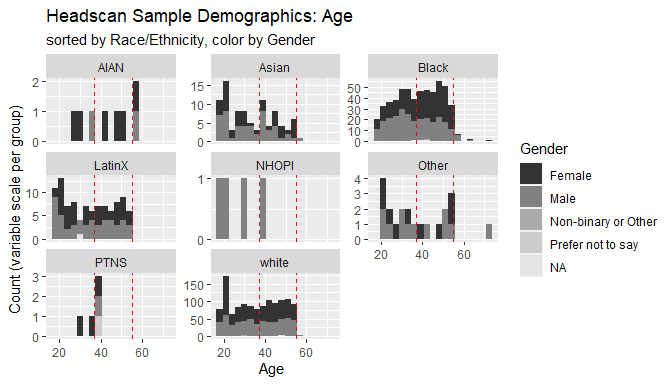
\includegraphics{demographic-data-exploration_files/figure-latex/unnamed-chunk-10-1.pdf}

\begin{Shaded}
\begin{Highlighting}[]
\CommentTok{\#ggplot(data=headscan\_full)+}
  \CommentTok{\#geom\_histogram(binwidth=2, aes(x=age, fill=race\_eth))+}
  \CommentTok{\#scale\_fill\_grey()+}
  \CommentTok{\#labs(title= "Demographics of Headscan Sample",}
       \CommentTok{\#subtitle = "Data collected by Human Solutions",}
       \CommentTok{\#fill= "Ethnicity",}
       \CommentTok{\#y="Count",}
       \CommentTok{\#x="Age")}
\end{Highlighting}
\end{Shaded}

\begin{Shaded}
\begin{Highlighting}[]
\CommentTok{\#ggplot(data=headscan\_full)+}
  \CommentTok{\#geom\_boxplot(aes(x=race\_eth, y=age, fill=gender))+}
  \CommentTok{\#scale\_fill\_grey()+}
  \CommentTok{\#theme(axis.text.x = element\_text(angle = 45))}
\end{Highlighting}
\end{Shaded}


\end{document}
